\documentclass[aspectratio=169]{beamer}
\usetheme{metropolis}
\usepackage{graphicx}
\usepackage{booktabs}
\usepackage{amsmath}
\usepackage[T1]{fontenc}
\usepackage[utf8]{inputenc}
\graphicspath{{../results/figures/}}

\title{Alveolar Epithelial Cells in Lethal COVID-19 Fan Out Along a Continuous Injury Axis}
\subtitle{Trajectory Analysis of SCP1219 with Ten-Way Ablation Robustness}
\author{[Author]}
\institute{Class Project}
\date{\today}

\begin{document}
\maketitle

\begin{frame}{What we asked}
\begin{itemize}
  \item Do alveolar epithelial cells in lethal COVID-19 fail as a coherent block, or as a continuous graded process?
  \item Pre-registered concept: \emph{epithelial robustness collapse}.
  \item Three pre-specified criteria:
  \begin{enumerate}
    \item Centroid displacement (one-sided Mann--Whitney $U$, COVID $>$ Healthy)
    \item Within-group dispersion (Levene)
    \item Pseudotime enrichment (1000-permutation test on median difference)
  \end{enumerate}
\end{itemize}
\end{frame}

\begin{frame}{Data}
\begin{itemize}
  \item Columbia/NYP COVID-19 Lung Atlas (SCP1219; Melms et al.\ 2021)
  \item 116{,}313 snRNA-seq nuclei $\rightarrow$ retained AT1/AT2/ECM-high epithelial $\rightarrow$ \textbf{22{,}128 cells}
  \item 9{,}608 AT1; 11{,}341 AT2; 1{,}179 ECM-high transitional
  \item 7 healthy (12{,}181 nuclei) + 20 COVID-19 donors (9{,}947 nuclei)
  \item Per-donor counts: 62 to 2{,}850 (10/27 donors $<$ 300 cells)
\end{itemize}
\end{frame}

\begin{frame}{Pipeline}
\begin{itemize}
  \item Scanpy 1.12.1 / anndata 0.12.10 / Python 3.12.3, seed 42
  \item Normalize $\rightarrow$ log1p $\rightarrow$ 3{,}000 HVGs (Seurat v3) $\rightarrow$ scale $\rightarrow$ 50-PC PCA
  \item $k$-NN ($k{=}15$) $\rightarrow$ UMAP, diffusion map (15 comp.)
  \item Diffusion pseudotime rooted at healthy-AT2 centroid, normalized to $[0,1]$
  \item 8 curated gene programs scored with \texttt{sc.tl.score\_genes}
  \item 10 pre-specified ablations
\end{itemize}
\alert{Harmony failed at runtime} (harmonypy returned shape (50,) instead of (22128,50)); pipeline fell back to uncorrected PCA.
\end{frame}

\begin{frame}{The manifold}
\centering
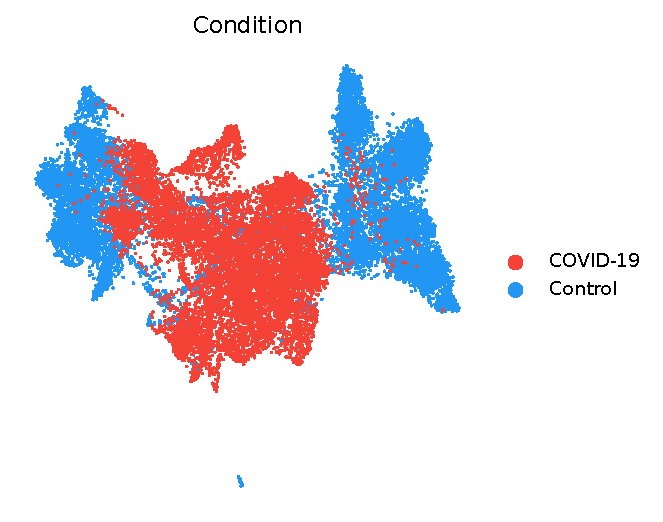
\includegraphics[width=0.45\linewidth]{fig1a_condition.pdf}\hfill
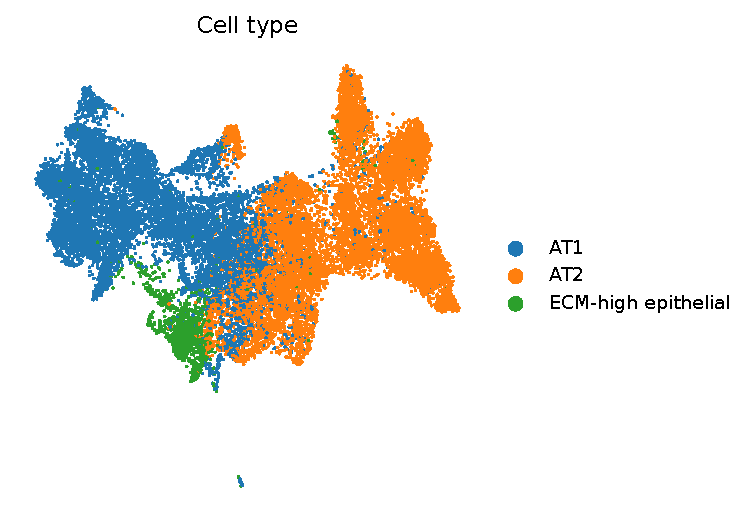
\includegraphics[width=0.45\linewidth]{fig1b_celltype.pdf}
\end{frame}

\begin{frame}{Pseudotime}
\centering
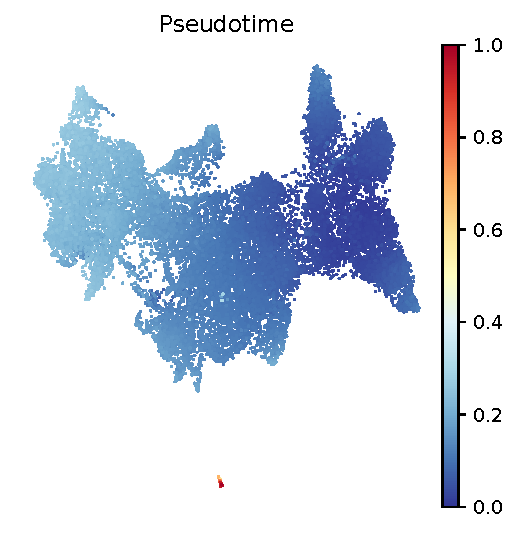
\includegraphics[width=0.7\linewidth]{fig2_pseudotime.pdf}
\end{frame}

\begin{frame}{Result 1 --- pseudotime shift}
\begin{itemize}
  \item Control median 0.063; COVID median 0.111; observed difference $+0.0483$
  \item 1{,}000-permutation null: mean $6.0\times10^{-5}$; std $1.24\times10^{-3}$
  \item Observed never exceeded in null $\Rightarrow$ $p = 0.000999$
  \item LOO (27 iters): direction preserved in \textbf{all 27}; range 0.028--0.202
  \item \alert{Magnitude is modest (4.8\% of the normalized axis).}
\end{itemize}
\centering
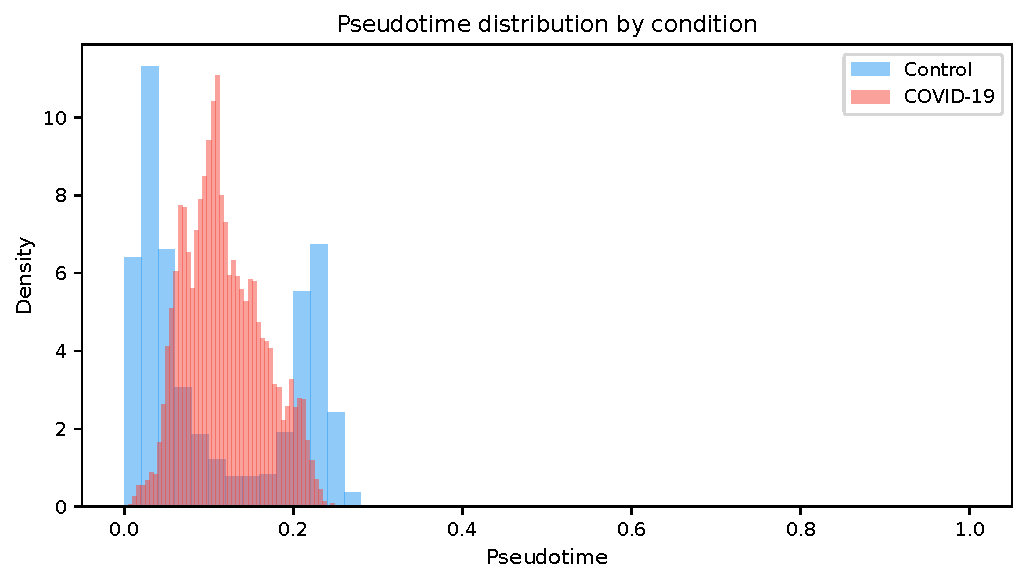
\includegraphics[width=0.55\linewidth]{fig4_pseudotime_density.pdf}
\end{frame}

\begin{frame}{Result 2 --- centroid displacement NOT supported}
\begin{itemize}
  \item One-sided Mann--Whitney $U$ in PCA-50 (COVID $>$ Healthy): $U = 5.21\times10^7$, $p = \textbf{1.0}$
  \item Means: COVID 12.36 vs.\ Healthy 12.10
  \item Medians: COVID \textbf{10.68} vs.\ Healthy \textbf{11.56} --- COVID median is \emph{lower}
  \item Rank-biserial $r = 0.14$ points opposite to the alternative
\end{itemize}
\alert{Pre-specified core test \textbf{failed}. We report this prominently.}
\end{frame}

\begin{frame}{Result 3 --- dispersion IS supported}
\begin{itemize}
  \item Within-group distance to own centroid, PCA-50
  \item Variance: COVID \textbf{33.28} vs.\ Healthy \textbf{14.58} (2.3-fold)
  \item Levene: statistic 276.5; $p < 10^{-30}$
\end{itemize}
\alert{COVID-19 cells are \emph{spread out}, not \emph{pushed away}.}
\end{frame}

\begin{frame}{Program ordering along pseudotime}
\centering
\small
\begin{tabular}{clll}
\toprule
Rank & Program & Peak & Peak score \\
\midrule
1 & AT2 identity & 0.015 & 0.75 \\
2 & AT1 identity & 0.266 & 1.25 \\
3 & Apoptosis & 0.591 & 0.17 \\
4 & AT2$\rightarrow$AT1 diff. & 0.744 & 0.57 \\
4 (tie) & NF-$\kappa$B & 0.744 & 0.18 \\
4 (tie) & Oxidative stress & 0.744 & 0.21 \\
7 & Interferon & 0.866 & 0.33 \\
8 & Senescence & 0.935 & 0.24 \\
\bottomrule
\end{tabular}
\\[4pt]
\alert{\textbf{Not} the hypothesized IFN$\rightarrow$NF-$\kappa$B$\rightarrow$repair$\rightarrow$apoptosis cascade.} Apoptosis peaks \emph{before} inflammatory/stress.
\end{frame}

\begin{frame}{Program dynamics}
\centering
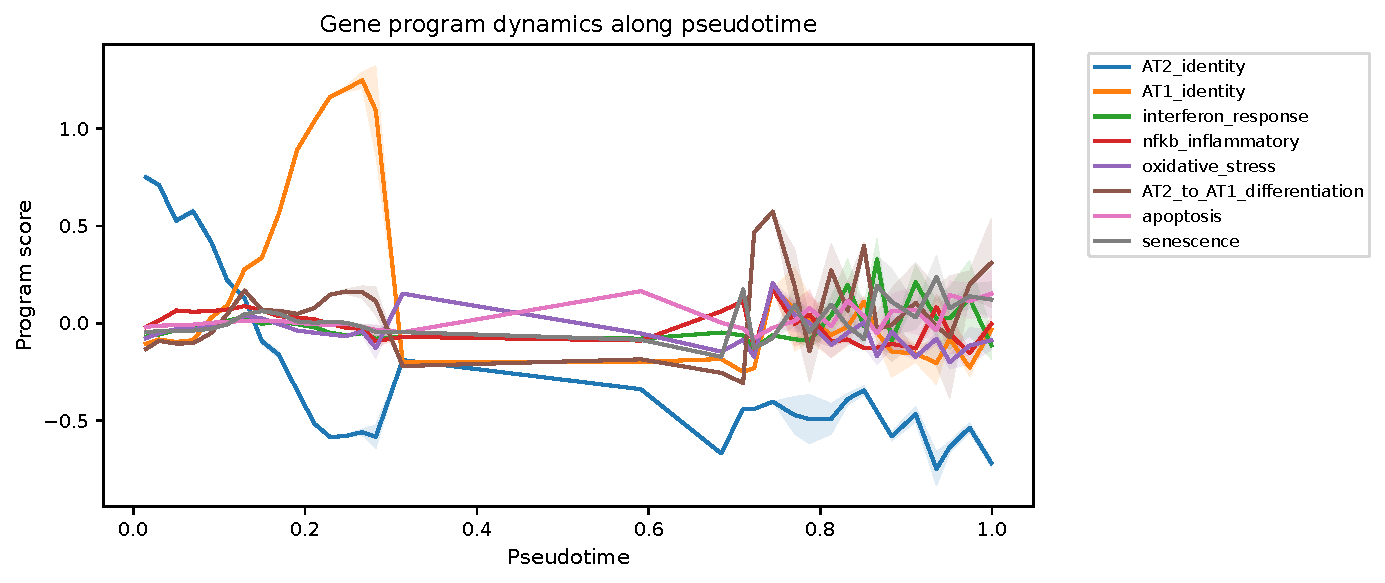
\includegraphics[width=0.8\linewidth]{fig3_program_dynamics.pdf}
\end{frame}

\begin{frame}{KRT8\textsuperscript{+} transitional cells}
\begin{itemize}
  \item 1{,}179 ECM-high / KRT8\textsuperscript{+}/CLDN4\textsuperscript{+} transitional cells
  \item \textbf{3.1$\times$ enriched in COVID-19}: 8.5\% vs.\ 2.7\%; $\chi^2$ $p < 10^{-30}$
  \item Intermediate pseudotime (mean 0.3--0.5)
  \item Concordant with DATP / aberrant-basaloid literature (Kobayashi 2020; Strunz 2020; Adams 2020; Habermann 2020)
  \item \alert{Correlational: snapshot, not lineage trace}
\end{itemize}
\end{frame}

\begin{frame}{Ten ablations --- summary}
\scriptsize
\begin{tabular}{lrrr l}
\toprule
Ablation & MPD & $\rho$ & $r$ & Notes \\
\midrule
1 AT2-only & $+0.133$ & 0.33 & $-0.29$ & sign flip on $r$ \\
2 UMAP / diffmap & $+0.048$ & 0.55 & $+0.14$ & unchanged \\
3 Harmony\textsuperscript{*} & $+0.048$ & 0.55 & $+0.14$ & \alert{both branches identical (Harmony failed)} \\
4 No apoptosis genes & $+0.074$ & 0.50 & $+0.14$ & slight up \\
5 4 roots & $-0.037$ to $+0.048$ & $-0.10$ to 0.64 & $+0.14$ & root-dependent \\
6 Broader epithelial & $-0.008$ & 0.83 & $+0.25$ & \alert{shift abolished} \\
7 LOO (27) & 0.028--0.202 & $-0.17$--0.74 & per-iter & direction preserved 27/27 \\
8 Curated-only & $+0.048$ & $1.00$ & $+0.14$ & stable \\
8 MSigDB-only & $+0.048$ & $-0.80$ & $+0.14$ & \alert{ordering inverted} \\
9 Palantir & --- & --- & --- & not installed \\
10 Permutation & $p=0.001$ & --- & --- & 1000 shuffles \\
\bottomrule
\end{tabular}
\end{frame}

\begin{frame}{Composite assessment}
\begin{tabular}{lr}
\toprule
Criterion & Outcome \\
\midrule
(1) Centroid displacement ($p < 0.05$) & \alert{\textbf{NOT supported}} ($p = 1.0$) \\
(2) Dispersion (Levene $p < 0.05$) & supported ($p \approx 0$) \\
(3) Pseudotime enrichment (perm.\ $p < 0.05$) & supported ($p = 0.001$) \\
\midrule
\textbf{Composite: \emph{moderate}} (2 of 3) & \\
\bottomrule
\end{tabular}
\end{frame}

\begin{frame}{What the data actually support}
\begin{itemize}
  \item Lethal COVID-19 \emph{fans out} alveolar epithelium along a continuous pseudotime axis.
  \item Signal is \textbf{loss of coherence}, not directional block displacement.
  \item KRT8\textsuperscript{+}/CLDN4\textsuperscript{+} transitional population accumulates at intermediate pseudotime (3.1$\times$ enriched) --- consistent with stalled AT2$\rightarrow$AT1 repair.
  \item The pseudotime shift is robust. The fine program ordering is \emph{hypothesis-generating}.
\end{itemize}
\end{frame}

\begin{frame}{What the data do NOT support}
\begin{itemize}
  \item Centroid displacement (pre-specified core test; $p=1.0$).
  \item A specific IFN$\rightarrow$NF-$\kappa$B$\rightarrow$repair$\rightarrow$apoptosis cascade (ordering inverts under MSigDB or COVID-extreme root).
  \item A pan-epithelial lung trajectory --- adding airway cells (Ablation 6) abolishes the shift.
  \item Any claim about elapsed time --- pseudotime is a manifold ordering, not a clock.
\end{itemize}
\end{frame}

\begin{frame}{Known limitations}
\begin{itemize}
  \item Cross-sectional, post-mortem, single dataset, lethal cases only.
  \item Donor imbalance: 10/27 donors $<$ 300 cells.
  \item Harmony failed $\Rightarrow$ Ablation 3 cannot distinguish corrected vs.\ uncorrected.
  \item Palantir not installed $\Rightarrow$ Ablation 9 no alt-trajectory comparison.
  \item GPX1 absent from HVGs (oxidative stress dropout); other programs unchecked.
  \item Fine ordering of injury programs sensitive to gene-list choice.
\end{itemize}
\end{frame}

\begin{frame}{Takeaways}
\begin{enumerate}
  \item Modest but robust pseudotime shift ($+0.048$, $p=0.001$).
  \item Significant dispersion increase ($2.3\times$ variance).
  \item Centroid displacement does not distinguish the conditions.
  \item KRT8\textsuperscript{+} transitional population $3.1\times$ enriched at intermediate pseudotime.
  \item Future robustness-collapse studies: use dispersion and trajectory metrics, not centroid displacement.
\end{enumerate}
\end{frame}

\begin{frame}[standout]
Questions?
\end{frame}

\end{document}
